%auto-ignore
\section{Experiments}
\label{sec:results}

Having detailed how to specify and optimize guide programs in our system, in this section, we experimentally evaluate how well programs written in our system can learn generative models and approximate posterior samplers. Unless stated otherwise, we use the following settings for the experiments in this section:
%%%
\begin{itemize}
\item{The Adam optimization method~\cite{Adam} with $\alpha = 0.1$, $\beta_1 = 0.9$, and $\beta_2 = 0.99$.}
\item{One sample from $\guide$ per optimization step to estimate the expectation in Equation~\ref{eq:finalEstimator}.}
\end{itemize}

\subsection{Gaussian Mixture Model}
\label{sec:results_gmm}

We first consider the simple Gaussian mixture model program from Figure~\ref{fig:bn_oneLatent} Bottom. This program samples discrete random choices, so its gradient estimator will include an LR term. Alternatively, we could re-write the program slightly to explicitly marginalize out the discrete random choices; see Appendix~\ref{sec:appendix_code:gmmSumOut}.
Marginalizing out of these choices leads to a tighter bound on the marginal log likelihood, so we would expect this version of the program to achieve a higher ELBo.
As a next your benefit, the gradient estimator for this program then reduces to the PW estimator, which will have lower variance. These benefits come at the cost of amortized inference, however, as this version of the program does not have a guide which can predict the latent cluster assignment given an observed point. We also consider a non-amortized, mean field version of the program for comparison.

Figure~\ref{fig:gmmResults} illustrates the performance of these programs after training for 200 steps on a synthetic datset of 100 points. On the left, we show how the ELBo changes during optimizaton.
As expected, ELBo progress asymptotes at a higher value for the marginalized model.
% Even on a simple model such as this one, the ability to use the pure PW estimator leads to faster convergence and a better final objective score.
On the right, we show the estimated negative log likelihood of a separate synthetic test set under each program after optimization. Here, we also include the true model (i.e. the model used to synthesize the test/training data) for comparsion.
As suggested by its optimization performance, the model with discrete choices marginalized out performs best.
Note that the amortized guide program slightly out-performs the mean field guide program, indicating that the generalization provided by amortization has benefits for training generative models, in addition to enabling fast predictions of latent variables for previously-unseen observations.

\begin{figure}[!ht]
\begin{minipage}{0.5\linewidth}
\centering
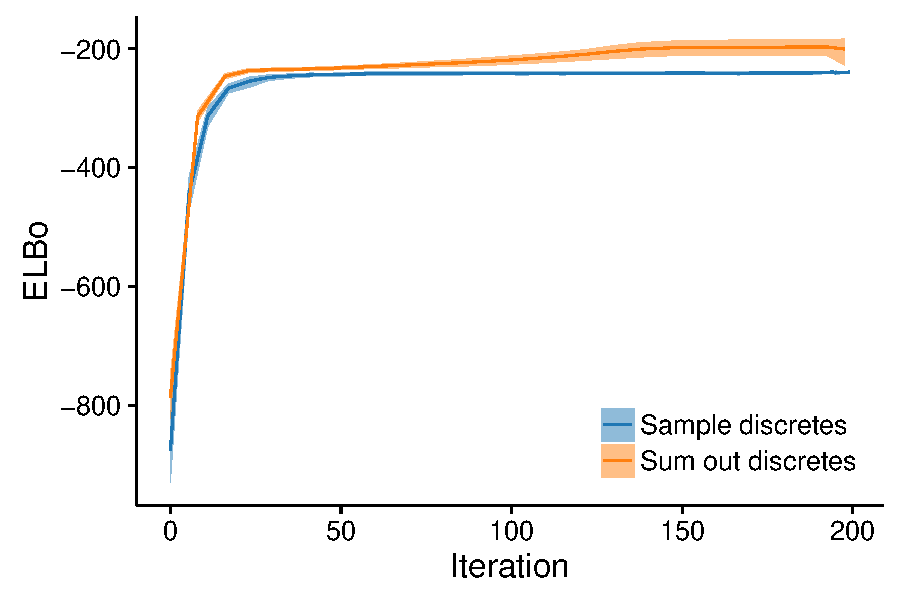
\includegraphics[width=\linewidth]{figs/results/gmm/elboProgress.pdf}
\end{minipage}
%
\begin{minipage}{0.5\linewidth}
\centering
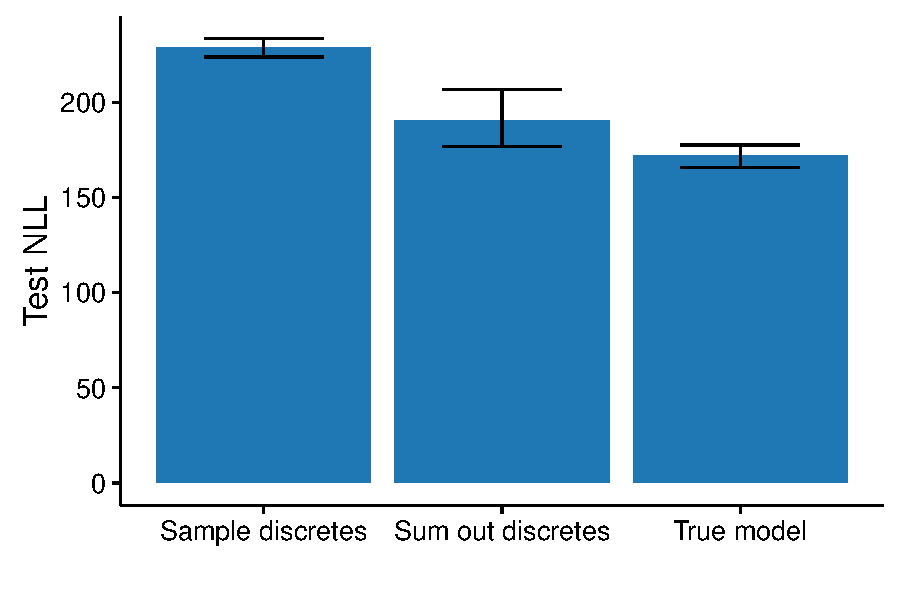
\includegraphics[width=\linewidth]{figs/results/gmm/nll.pdf}
\end{minipage}
\caption{Performance of simple Gaussian mixture model program. \emph{(Left)} ELBo optimization progress during training. The optimization objective for the marginalized model is a tighter bound on the marginal log likelihood and thus has a higher asymptote. \emph{(Right)} Negative log-likelihood of a held-out test set.}
\label{fig:gmmResults}
\end{figure}

% Other Bayes net examples??

\subsection{QMR-DT}
\label{sec:results_qmr}

We next consider a more complicated Bayesian network model based on the QMR-DT medical diagnosis network~\cite{QMR}. QMR-DT is a bipartite graphical model with one layer of nodes corresponding to latent causes (e.g. diseases, in the medical setting) and a second layer of observed effects (e.g. symptoms). All nodes are binary (i.e. Bernoulli), and the cause nodes are connected to the effects via directed noisy-or links. Appendix~\ref{sec:appendix_code:qmr} shows our implementation.

Our amortized guide program for this model uses a neural network to jointly predict the probabilities of all latent cause variables given a set of observed effects. Since the QMR-DT model contains a large number of discrete random variables, we expect the variance reduction strategies introduced in Section~\ref{sec:optimization:unifiedEstimator} to have significant effect.
Thus, we consider training this guide program with no variance reduction (\emph{Amortized}, step size $10^{-5}$), with per-choice likelihood ratio weights, (\emph{+ local weights}, step size $10^{-3}$), and with both per-choice weights and baselines (\emph{+ baselines}, step size $10^{-2}$). As a point of reference, we also include a mean field model (step size $10^{-2}$) which uses all variance reduction strategies.
Data for our experiments is sampled from a randomly-generated graph with 200 causes and 100 effects. We sample 1000 observations for the training set and an additional 100 for a held-out test set.
% \ndg{note that the fully-marginalized approach isn't really tractable anymore due to the size of the latent space?}

Figure~\ref{fig:qmrResults} shows the results of our experiments. The left plot shows optimization progress under each condition. Without any of the variance reduction strategies, gradients are extremely noisy and optimization makes almost no progress. Using local, per-variable likelihood ratio weights allows optimization to mke progress, and adding per-variable baselines further boosts performance. Though it uses all variance reduction strategies, the mean field model trains significantly more slowly than the variance-reduced amortized models. This happens because the mean field model has separate parameters for each training observation, rather than a single parameter set shared by a neural network, i.e. it has many more parameters that are each updated by very few gradient steps. Amortization thus both facilitates fast posterior prediction and exhibits faster training due to parameter sharing.

We next evaluate the guide program's posterior prediction ability. We use the learned guide to sample latent causes given an observed set of effects from the test set, sample effects given those causes, and then record what percentage of active effects in the test set observation are correctly predicted by the effects `hallucinated' from our model. Specifically, if $\vecstyle{e}$ is a vector of effect variables of length $N$, then the metric we use is:
%%%
\begin{align*}
&\min(F(\vecstyle{e}_{\text{true}}, \vecstyle{e}_{\text{sampled}}), F(\vecstyle{e}_{\text{sampled}}, \vecstyle{e}_{\text{true}}))\\
&F(\vecstyle{e}_1, \vecstyle{e}_2) = \frac{1}{\sum_i^N \vecstyle{e}_1(i)} \sum_{i, \vecstyle{e}_1(i) = 1} \indicator{\vecstyle{e}_2(i) = 1}
\end{align*}
%%%
where $\vecstyle{e}_{\text{true}}$ are effects from the test set and $\vecstyle{e}_{\text{sampled}}$ are hallucinated from the model.
Figure~\ref{fig:qmrResults} Right plots the average $F$ score over 100 runs, where we compare our amortized guide program against using the prior program to sample latent causes. The learned guide program correctly predicts more than twice as many active effects.

\begin{figure}[!ht]
\begin{minipage}{0.6\linewidth}
\centering
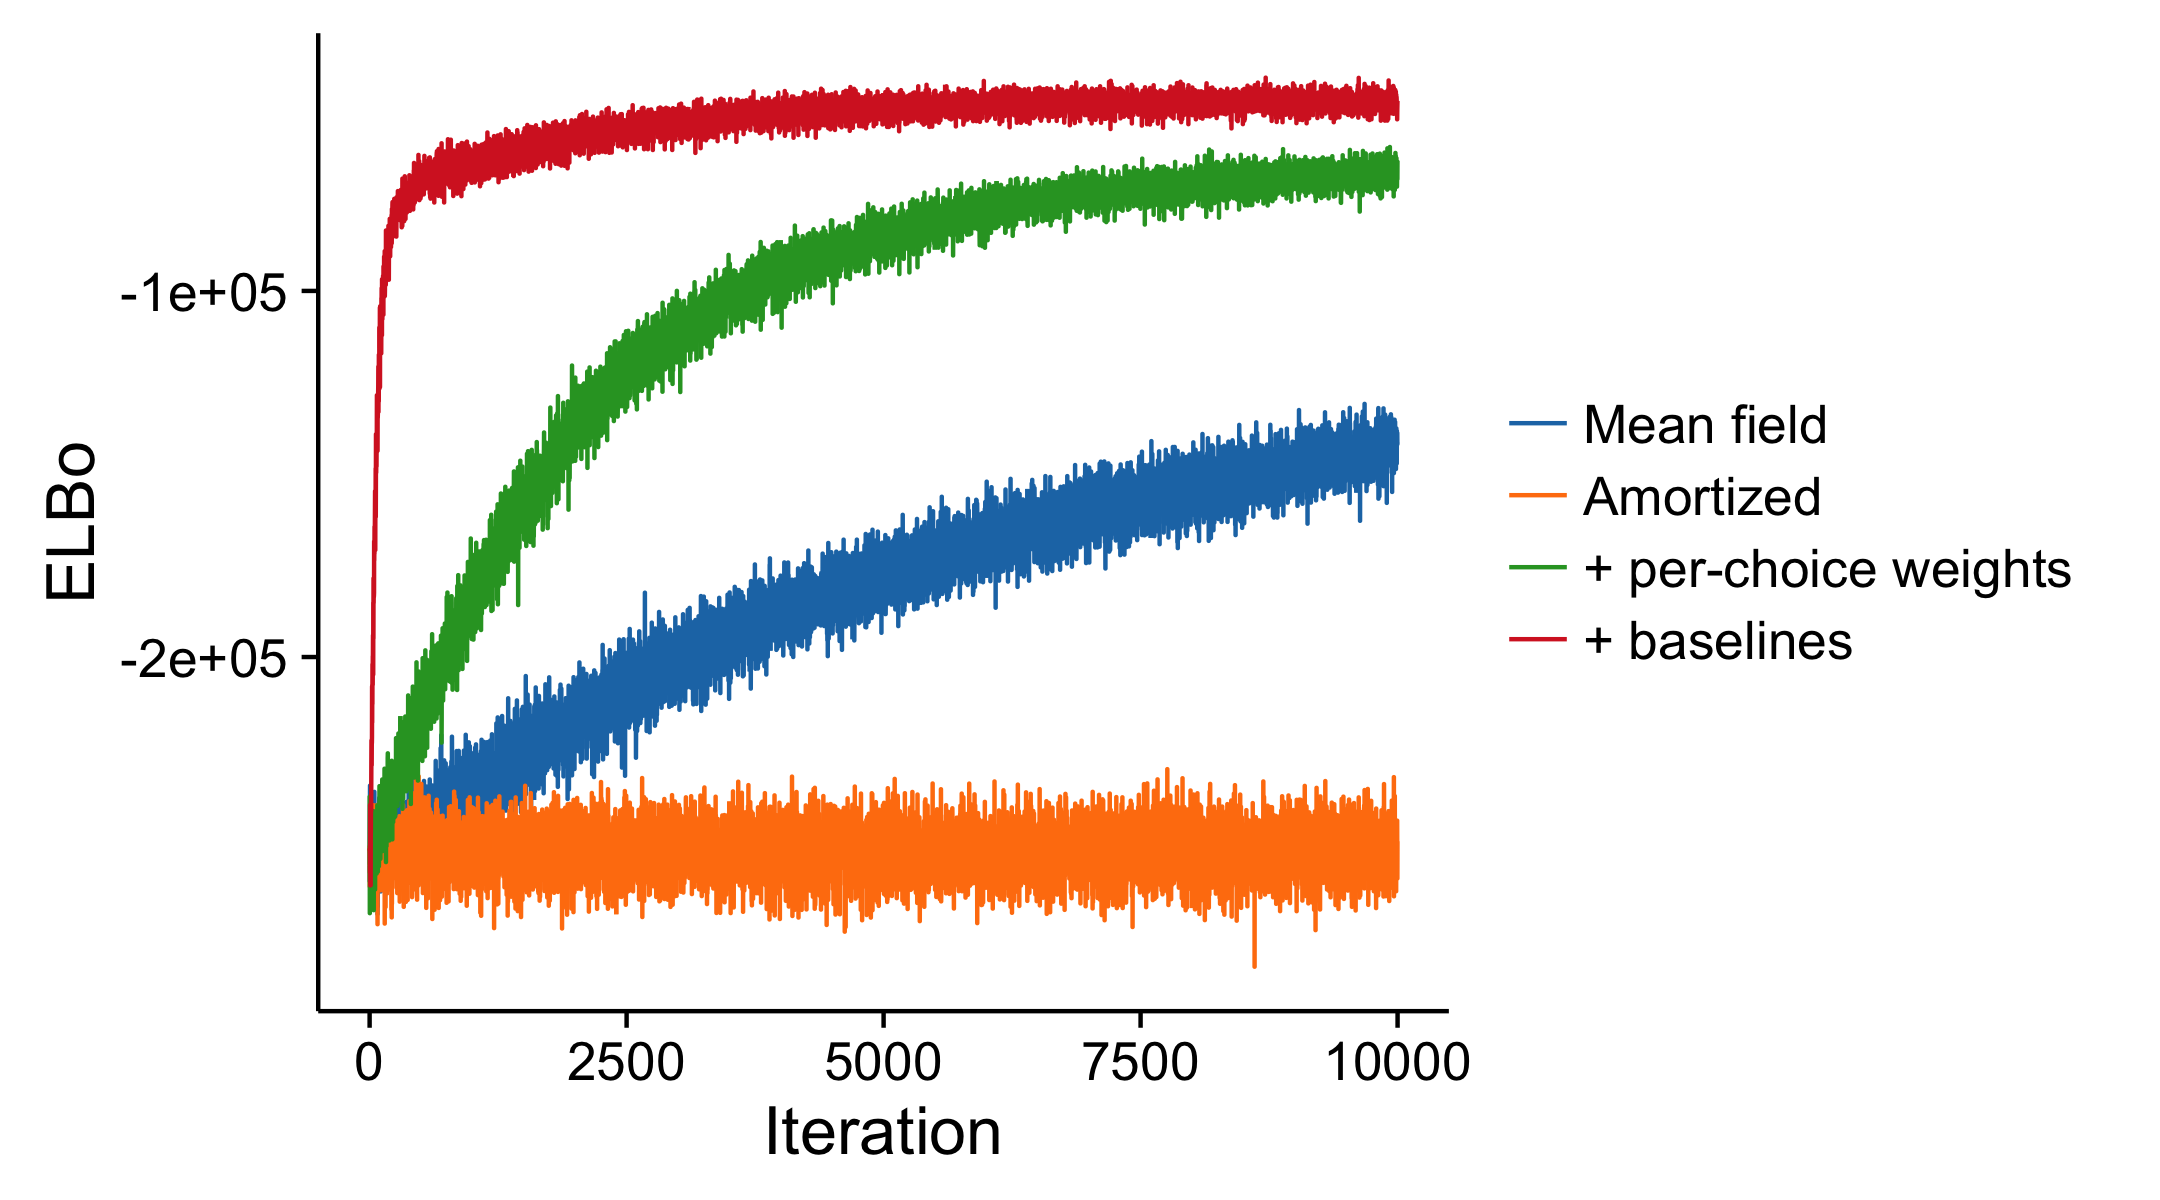
\includegraphics[width=\linewidth]{figs/results/qmr/elboProgress.png}
\end{minipage}
%
\begin{minipage}{0.4\linewidth}
\centering
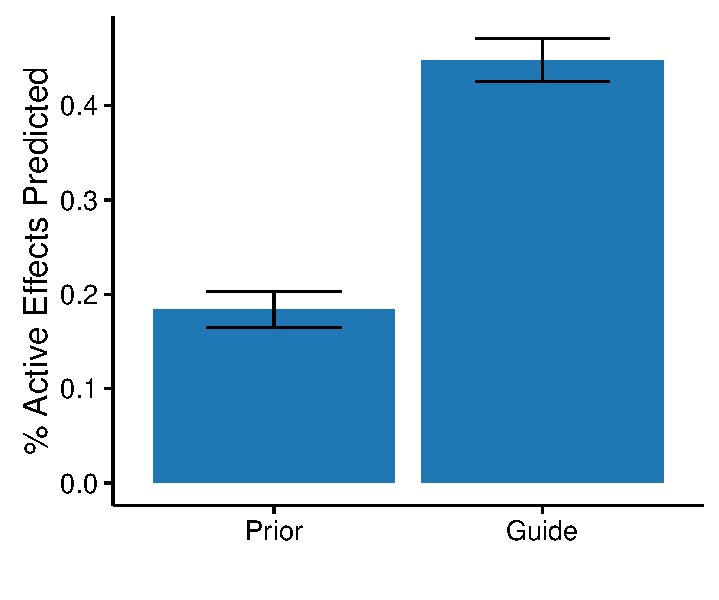
\includegraphics[width=\linewidth]{figs/results/qmr/reconstructScores.pdf}
\end{minipage}
\caption{Performance of a QMR-DT model. \emph{(Left)} ELBo optimization progress during training. \emph{(Right)} Percentage of test set active effects correctly predicted using latent causes sampled from either the prior or the guide program.}
\label{fig:qmrResults}
\end{figure}

In addition to the guide program described above, which predicts all latent causes jointly given the observed effects, we also experimented with `factored' guide programs which predict each latent cause one-by-one given the observed effects. We consider a guide that predicts each latent cause independently (\emph{Factored}), as well as a guide that introduces dependencies between all latent causes via a recurrent neural network (\emph{Factored + GRU}). The recurrent network receives as input the value of each latent cause as it is sampled, maintaining a persistent hidden state  that, in theory, can capture the values of all latent causes sampled thus far. We use the gated recurrent unit (GRU) architecture for its ability to capture a longer-range dependencies~\cite{GRU}, with a hidden state of dimension 20. The code for these programs is shown in Appendix~\ref{sec:appendix_code:qmr}.
We use stepsize 0.01 for both during optimization.

Figure~\ref{fig:qmrResults_factored} compares these guide programs with the joint guide used earlier in this section.
While the independent factored guide performs slightly less well than the joint guide, adding the recurrent neural network to capture posterior dependencies improves performance to slightly better than the joint guide.
One caveat is that the \emph{Factored + GRU} guide takes significantly longer to train in our implementation due to the recurrent network computation.
Later in the paper, we discuss how this guide structure might point the way toward automatically deriving guide programs.

\begin{figure}[!ht]
\begin{minipage}{0.5\linewidth}
\centering
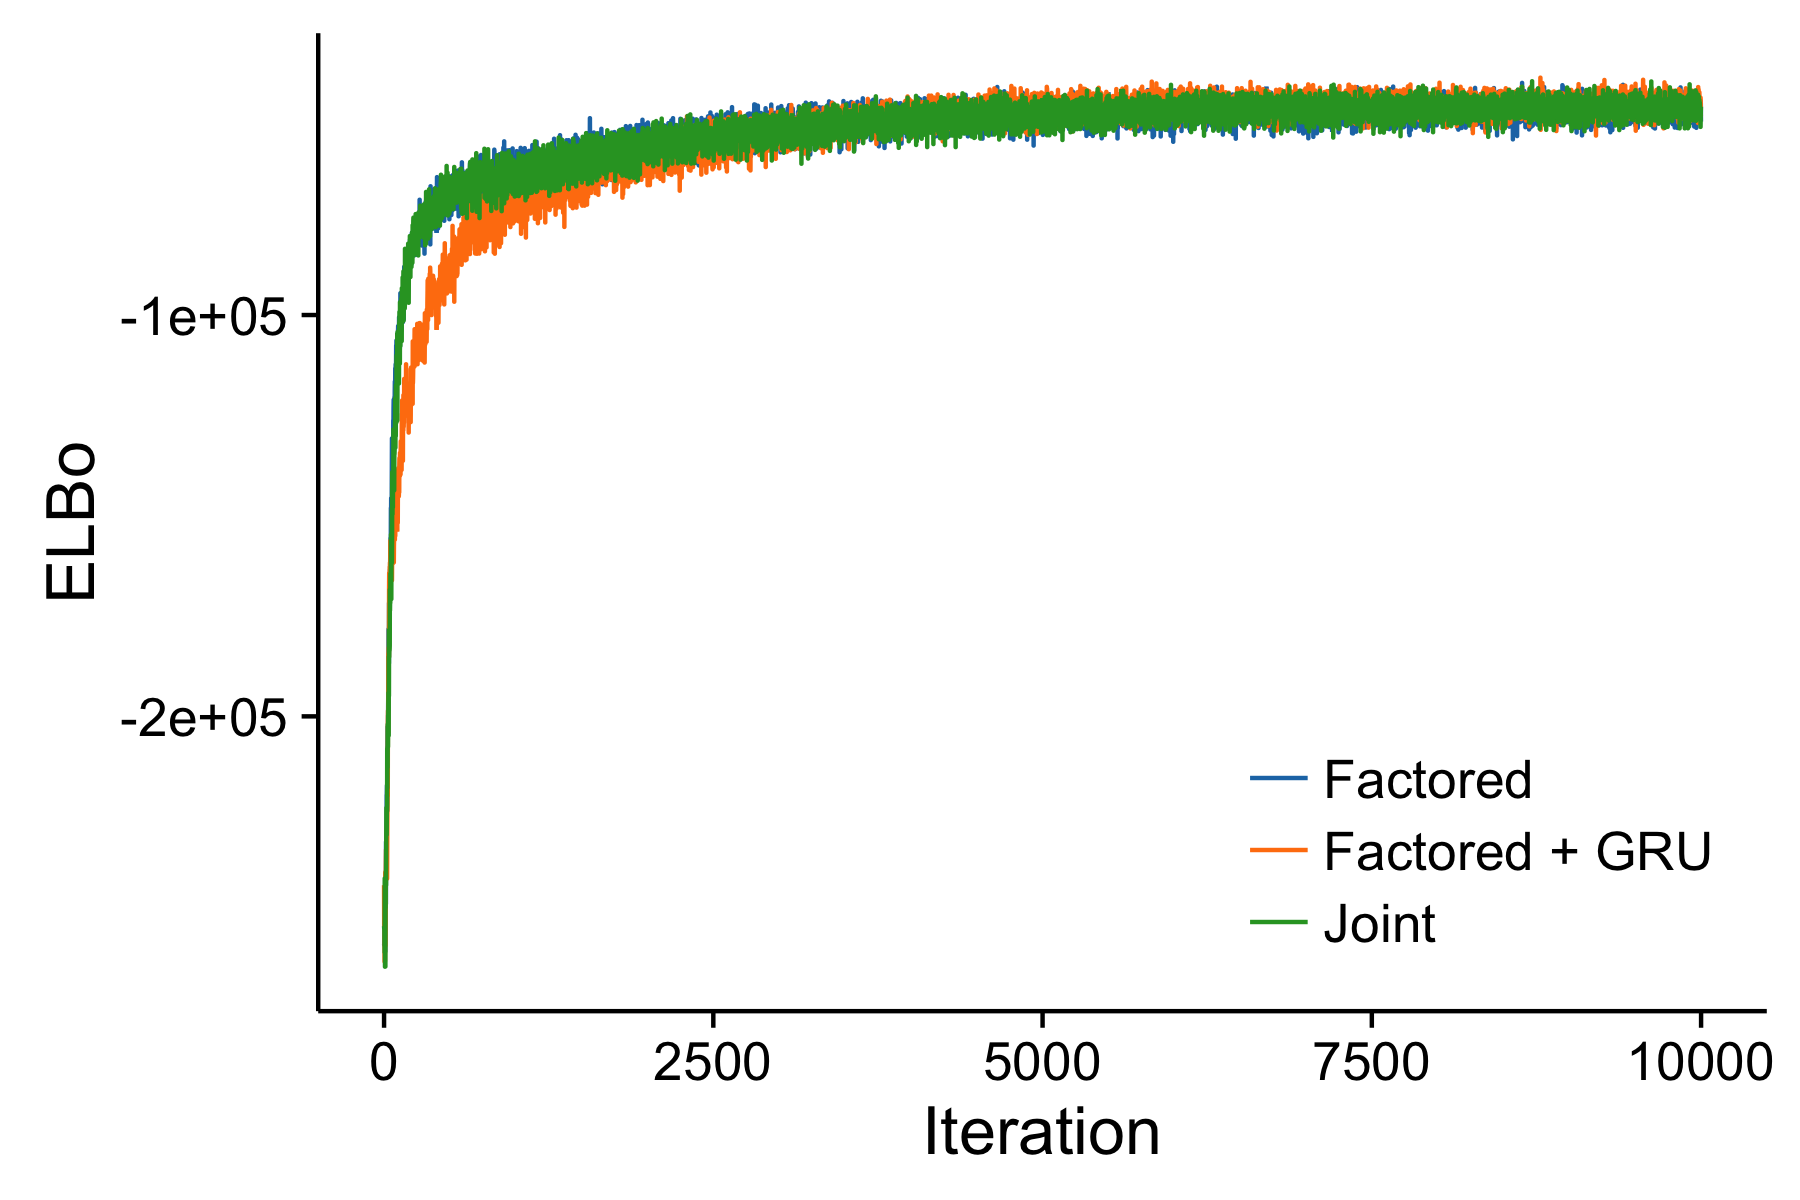
\includegraphics[width=\linewidth]{figs/results/qmr/elboProgress_factored.png}
\end{minipage}
%
\begin{minipage}{0.5\linewidth}
\centering
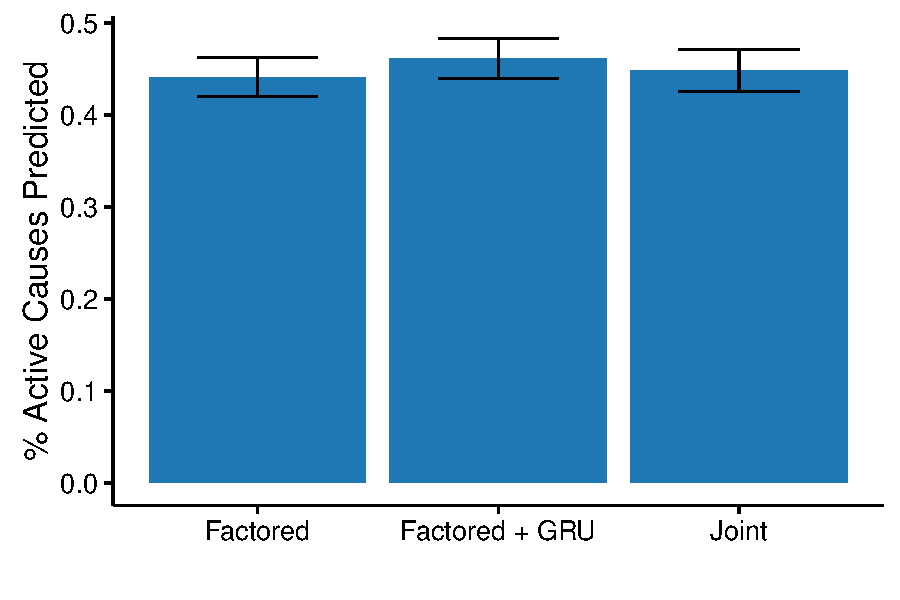
\includegraphics[width=\linewidth]{figs/results/qmr/reconstructScores_factored.pdf}
\end{minipage}
\caption{Experimenting with factored guide programs for QMR-DT. \emph{(Left)} ELBo optimization progress during training. \emph{(Right)} Percentage of test set active effects correctly predicted using latent causes sampled from either the prior or the guide program.}
\label{fig:qmrResults_factored}
\end{figure}


%\ndg{TODO: it'd be great to show an example of how daipp can handle missing evidence. currently observe defaults to sample when the val is undefined (i think). so we need to make sure that observe passes its options arg through to this sample. then we can add a guide to the observes. simplest might be an RNN that runs across the observes predicting them, before using the net to predict latents. hmm, we'll want to incorporate observed data in the data-predictor net... so need to have observe to something for defined vals as well.
%
%actually, there's no reason to predict the missing observe values (unless we care about them): we can run an rnn over the observations (with address so we know which is which) to build an 'observation vector' then predict the latents from this.}

\subsection{Latent Dirichlet Allocation}
\label{sec:results_lda}

We also used our system to implement amortized inference in Latent Dirichlet Allocation topic models, over a data set of abstracts taken from the Stanford Computation and Cognition Lab's publication page.\footnote{Thanks to Robert Hawkins for creating this dataset.}

We experimented with two different amortized guide programs.
The first is local to each word in a document (\emph{Word-level guide}): it learns to predict the latent topic for each word, given the word and the latent topic distribution for the document.
The second is local to each document (\emph{Document-level guide}): it learns to predict the latent topic distribution for the document, given the words in the document and the latent word distributions for each topic.
These two guides support amortized inference at different granularities and thus have different parameter sharing characteristics, which may lead to different learning behavior.
For comparison, we also included two non-amortized conditions: a mean field model, and a mean field model with the latent choice of topic per word marginalized out (\emph{Marginalized mean field}).
Code for all of these programs can be found in Appendix~\ref{sec:appendix_code:lda}.
We use five topics and learning rate 0.01 in all experiments.

Figure~\ref{sec:results_lda} shows the results of these experiments.
In the optimization progress plot on the left, we see that the marginalized mean field model achieve the highest ELBo.
This is consistent with the results from the Gaussian mixture model experiments: marginalizing out latent variables when possible leads to a tighter bound on the marginal log likelihood.
% In the ELBo progress plot on the left, we see that the marginalized mean field model converges fastest: this is consistent with the result from the Gaussian mixture model experiments and further emphasizes the performance benefits of eliminating discrete random choices when possible.

Of our two amortized guides, the word-level guide performs better (and nearly as well as the marginalized model), likely due to increased parameter sharing. The document-level guide performs at least as well as the mean field model while also being able to efficiently predict topic distributions for previously-unseen documents.

Figure~\ref{sec:results_lda} Right shows the top ten highest probability words in each inferred topic for the marginalized mean field model. From left to right, these topics appear to be about experiments, pragmatic language models, knowledge acquisition, probabilistic programming languages, and a grab bag of remaining topics.

\begin{figure}[!ht]
\begin{minipage}{0.5\linewidth}
\centering
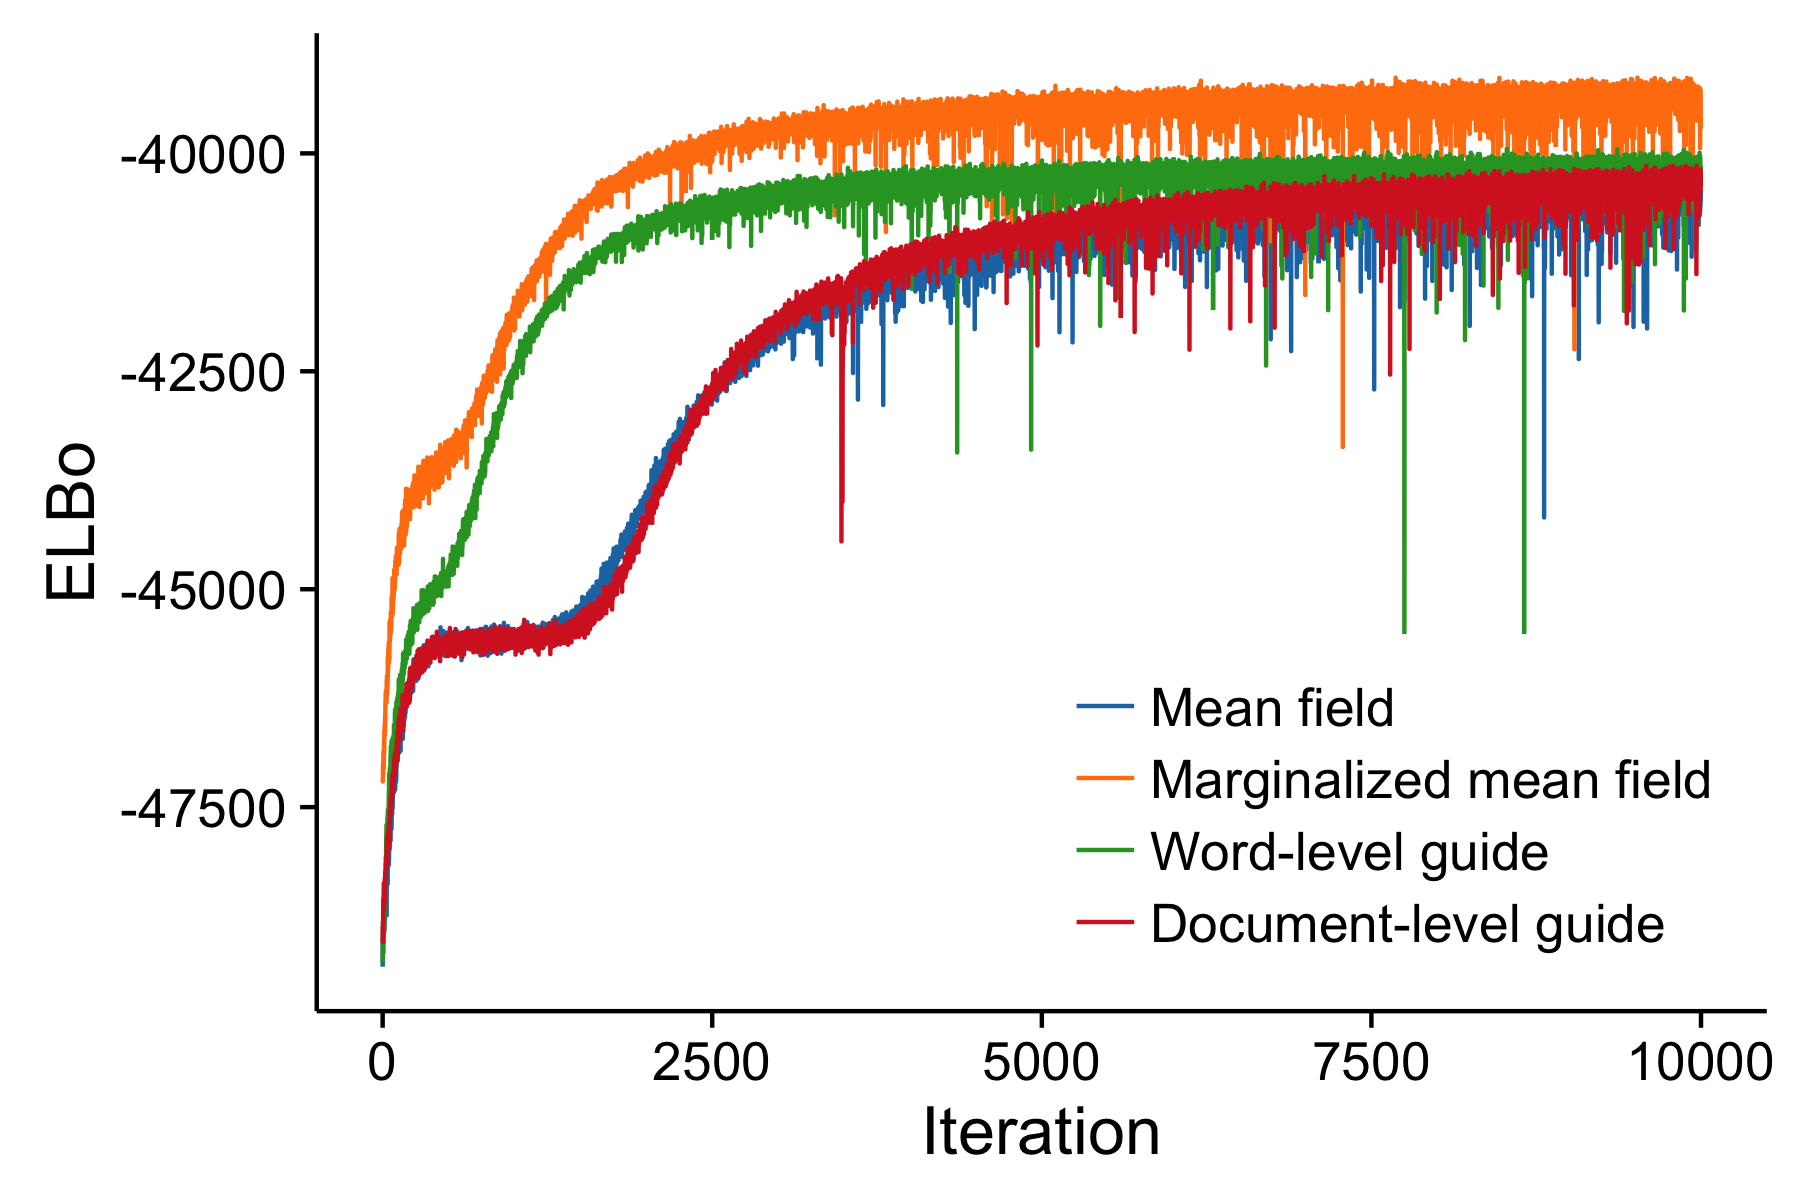
\includegraphics[width=\linewidth]{figs/results/lda/elboProgress.png}
\end{minipage}
%
\begin{minipage}{0.5\linewidth}
\tiny
\centering
\begin{tabular}{c c c c c}
\textbf{Topic 1} & \textbf{Topic 2} & \textbf{Topic 3} & \textbf{Topic 4} & \textbf{Topic 5}\\
model & model & loop & probabilistic & attempt\\
causal & language & learning & models & inference\\
dynamic & pragmatic & abstract & programming & novel\\
judgments & abstract & extension & church & decisions\\
evidence & interpretation & bayesian & abstract & required\\
abstract & inference & knowledge & using & models\\
actions & knowledge & human & inference & behavior\\
pedagogical & words & causal & stochastic & bayesian\\
people & form & theories & language & cognition\\
participants & using & theory & model & expressive
\end{tabular}
\end{minipage}
%
\caption{Performance of Latent Dirichlet Allocation models. \emph{(Left)} ELBo optimization progress during training. The optimization objective for the marginalized model is a tighter bound on the marginal log likelihood and thus has a higher asymptote. \emph{(Right)} Top ten highest probability words in each inferred topic for the best-performing model.}
\label{fig:ldaResults}
\end{figure}

\subsection{Neural Generative Models: Variational Autoencoder \& Sigmoid Belief Network}
\label{sec:results_vae}

Our system naturally supports generative models which use neural network components. Two prominent examples of models in this class include the Variational Autoencoder (VAE) and Sigmoid Belief Networks (SBN). Both models sample latent variables from a multivariate distribution and then transform the result via a neural network to produce observed variables, often in the form of an image. The VAE uses a latent multivariate Gaussian distribution, whereas the SBN uses a latent multivariate Bernoulli.

Appendix~\ref{sec:appendix_code} shows implementations of these models in our system. Our VAE implementation follows the original description of the model by Kingma and Welling~\cite{AEVB}, and our SBN implementation follows that of Mnih and Gregor~\cite{NVIL}.
The VAE uses a 20-dimensional latent code, and the SBN uses a single layer of 200 hidden variables. Our system cannot express the two-layer SBN of Mnih and Gregor, because its guide model samples the latent variables in the reverse order of the generative model.

Figure~\ref{fig:vae_sbn_results} Left shows results of training these models on the MNIST dataset, using Adam with a step size of 0.001.
While both models train quickly at first, the SBN's training slows more noticeably than the VAE's due to its discrete nature. It takes more than three times as many iterations to achieve the same ELBo.
In Figure~\ref{fig:vae_sbn_results} Right, we qualitatively evaluate both models by using them to reconstruct images from the MNIST test set. We use the guide program to sample latent variables conditional on the images in the ``Target'' column (i.e. the `encoder' phase). We then transform these latent variables using the generative model's neural networks (i.e. the `decoder' phase) to produce the reconstructed images in the ``VAE'' and ``SBN'' columns.
As suggested by their training behavior, the VAE is able to generate higher-quality reconstructions after less training.

Our optimization exhibits some differences from the previous work.
For the VAE, Kingma and Welling~\cite{AEVB} exploit the closed-form solution of the KL divergence between two Gaussians to create an even lower-variance estimator of the ELBo gradient. We use a more general formulation, but our system can still successfully train the model.
For the SBN, Mnih and Gregor~\cite{NVIL} use neural networks to compute the per-variable baselines $b_i$ in Equation~\ref{eq:finalEstimator}, whereas we use a simpler approach (see Appendix~\ref{sec:appendix_proofs}).
However, the key point is that each of these models was described in a simple WebPPL program with neural guides and optimized by the default system, without the need for additional implementation efforts.

\begin{figure}
\begin{minipage}{0.5\linewidth}
\centering
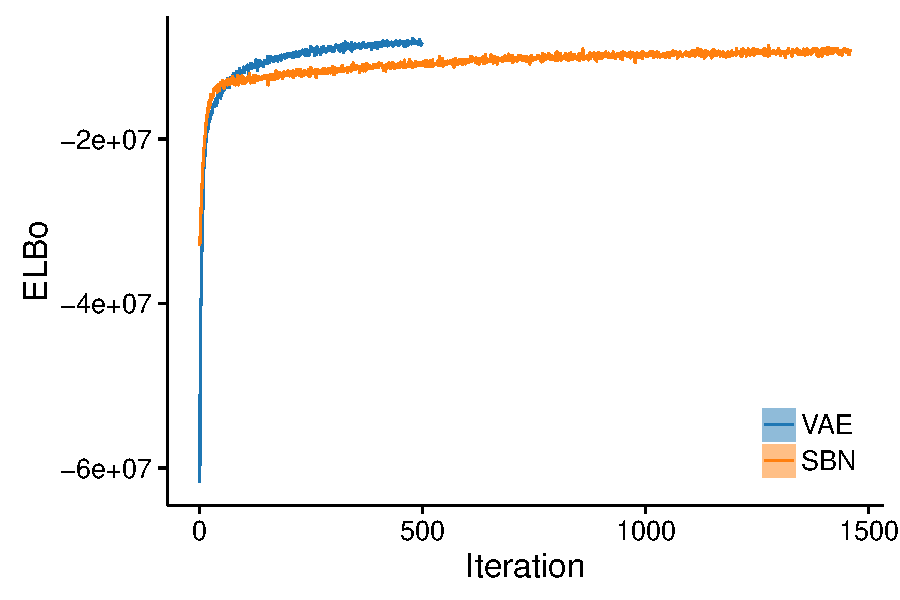
\includegraphics[width=\linewidth]{figs/results/vae_sbn/elboProgress.pdf}
\end{minipage}
%
\hspace{2em}
%
\begin{minipage}{0.5\linewidth}
\setlength{\tabcolsep}{1pt}
\centering
\begin{tabular}{c  c c c c c c}
Target & \multicolumn{3}{c}{VAE} & \multicolumn{3}{c}{SBN}
\\
 
\includegraphics[width=0.12\linewidth]{figs/results/vae_sbn/vae_encodeDecode_target_000.png}
 \hspace{3pt}
& 
\includegraphics[width=0.12\linewidth]{figs/results/vae_sbn/vae_encodeDecode_target_000_sample_001.png}
& 
\includegraphics[width=0.12\linewidth]{figs/results/vae_sbn/vae_encodeDecode_target_000_sample_002.png}
& 
\includegraphics[width=0.12\linewidth]{figs/results/vae_sbn/vae_encodeDecode_target_000_sample_003.png}
\hspace{3pt}
& 
\includegraphics[width=0.12\linewidth]{figs/results/vae_sbn/sbn_encodeDecode_target_000_sample_001.png}
& 
\includegraphics[width=0.12\linewidth]{figs/results/vae_sbn/sbn_encodeDecode_target_000_sample_002.png}
& 
\includegraphics[width=0.12\linewidth]{figs/results/vae_sbn/sbn_encodeDecode_target_000_sample_003.png}
\\
 
\includegraphics[width=0.12\linewidth]{figs/results/vae_sbn/vae_encodeDecode_target_001.png}
 \hspace{3pt}
& 
\includegraphics[width=0.12\linewidth]{figs/results/vae_sbn/vae_encodeDecode_target_001_sample_001.png}
& 
\includegraphics[width=0.12\linewidth]{figs/results/vae_sbn/vae_encodeDecode_target_001_sample_002.png}
& 
\includegraphics[width=0.12\linewidth]{figs/results/vae_sbn/vae_encodeDecode_target_001_sample_003.png}
\hspace{3pt}
& 
\includegraphics[width=0.12\linewidth]{figs/results/vae_sbn/sbn_encodeDecode_target_001_sample_001.png}
& 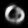
\includegraphics[width=0.12\linewidth]{figs/results/vae_sbn/sbn_encodeDecode_target_001_sample_002.png}
& 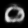
\includegraphics[width=0.12\linewidth]{figs/results/vae_sbn/sbn_encodeDecode_target_001_sample_003.png}
\\
 
\includegraphics[width=0.12\linewidth]{figs/results/vae_sbn/vae_encodeDecode_target_002.png}
 \hspace{3pt}
& 
\includegraphics[width=0.12\linewidth]{figs/results/vae_sbn/vae_encodeDecode_target_002_sample_001.png}
& 
\includegraphics[width=0.12\linewidth]{figs/results/vae_sbn/vae_encodeDecode_target_002_sample_002.png}
& 
\includegraphics[width=0.12\linewidth]{figs/results/vae_sbn/vae_encodeDecode_target_002_sample_003.png}
\hspace{3pt}
& 
\includegraphics[width=0.12\linewidth]{figs/results/vae_sbn/sbn_encodeDecode_target_002_sample_001.png}
& 
\includegraphics[width=0.12\linewidth]{figs/results/vae_sbn/sbn_encodeDecode_target_002_sample_002.png}
& 
\includegraphics[width=0.12\linewidth]{figs/results/vae_sbn/sbn_encodeDecode_target_002_sample_003.png}
\\
 
\includegraphics[width=0.12\linewidth]{figs/results/vae_sbn/vae_encodeDecode_target_003.png}
 \hspace{3pt}
& 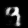
\includegraphics[width=0.12\linewidth]{figs/results/vae_sbn/vae_encodeDecode_target_003_sample_001.png}
& 
\includegraphics[width=0.12\linewidth]{figs/results/vae_sbn/vae_encodeDecode_target_003_sample_002.png}
& 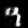
\includegraphics[width=0.12\linewidth]{figs/results/vae_sbn/vae_encodeDecode_target_003_sample_003.png}
\hspace{3pt}
& 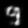
\includegraphics[width=0.12\linewidth]{figs/results/vae_sbn/sbn_encodeDecode_target_003_sample_001.png}
& 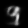
\includegraphics[width=0.12\linewidth]{figs/results/vae_sbn/sbn_encodeDecode_target_003_sample_002.png}
& 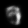
\includegraphics[width=0.12\linewidth]{figs/results/vae_sbn/sbn_encodeDecode_target_003_sample_003.png}
\end{tabular}
\end{minipage}
\caption{Evaluating the Variational Autoencoder (VAE) and Sigmoid Belief Network (SBN) programs on the MNIST dataset. \emph{(Left)} ELBo optimization progress during training. \emph{(Right)} Reconstructing the images in the ``Target'' column using both models.}
\label{fig:vae_sbn_results}
\end{figure}


%Things to try if we have time:
%\begin{itemize}
%\item{Simple bayesian NN (show how easy it is to do full variational Bayes)}
%\item{HMM-type families: Deep kalman filter? Or other RNN VAE type thing?}
%\item{PCFG (prob won’t work, but useful to understand). Continuous feature-passing version?}
%\end{itemize}
%
